\documentclass[12pt]{article}
\usepackage[utf8]{inputenc}
\usepackage{graphicx, latexsym, amsmath, amssymb, amsthm}
\usepackage{multicol}
\usepackage{geometry}
 \geometry{
 a4paper,
 total={170mm,257mm},
 left=16mm,
 top=10mm,
 }

\graphicspath{{../apps/aco_tsp/test/results/}}
\title{Ant Colony Optimization in Elixir}
\author{Andrea Malleo}
\begin{document}

\maketitle
\section{Abstract}
In this paper we present a distributed implementation of an Ant Colony Optimizer 
for the Travelling Salesman problem using the Actor Model of Concurrency. We give
an overview of the system architecture and present the experiments we ran to validate 
the correctness of the code and compare performance against an open source serialized 
implementation. We find that performance compared to the serialized approach scales 
with the problem size, and identify key future enhancements for further speed up.

%\begin{multicols*}{2}

\section{Introduction}Ant Colony Optimization \cite{Dorigo1997AntCS} is a bio-inspired coorperative learning algorithm for 
    finding the shortest path in a graph. Ants are simulated as software agents who 
    independently travel along the graph, dropping pheromones in their wake that 
    evaporate with time. These pheromones are a form of communication for other ants in
    the colony, as concentration of pheromones on a pathway signals recent ant traffic. \\

    The algorithm is iterative, and each ant completes a tour every round.
    After each round, the solutions for each of the ants are aggregated
    and the optimal choice from all of the candidates is selected. 
    Additionally the shared pheromone matrix, acting as a collective and evolving intelligence 
    for the colony of ants, is updated to reflect new pheromone concentrations following all of the 
    ant tours of this round.  In successive rounds of the algorithm, ants bias their path 
    toward edges with higher pheromone concentration. Since edges of greater distance take 
    longer to travel, evaporation will lower the concentration of pheromone there and make 
    future ants less likely to take those edges. Over successive rounds, the searches converge
    to some (locally) optimal solution. 
    There have since been many enhancements to the original Any Colony algorithm,
    such as the Ant Colony System \cite{Dorigo1999AntCO} and the Max-Min Ant System \cite{maxMin} 
    which produce better convergence results. In this paper we stuck with the original, simplest 
    approach and settled for convergence to some local minimum which empirically proved to be 
    not too far from the global minimum.\\

    The problem being considered here is the Travelling Salesman Problem \cite{wikiTSP},
    that is to find a complete tour of a fully connected graph with minimal 
    cost.


\section{Related work}
The independence of the ant agents lends the algorithm to parallelization. 
The central point of synchronization is the pheromone matrix, which must 
maintain accurate values for a given round and update atomically for the 
next round. Many approaches have been presented that parallelize the algorithm 
in different ways. Pedemonte et. al \cite{SurveyParallel} categorize 
the approaches, drawing distrinctions between a *master-slave model*
with the simultaneous execution of ants providing updates to 
a master process maintainting the global pheromone matrix and a
*parallel independent runs model* where many
executions of independent ACO systems run simultaneously,
further subdivided between
whether or not the independent colony systems eventually coordinate
 with each other. 
There are also GPU based implementations, such as in \cite{GPU}.
\\

Instead of working under the shared memory model of distributed 
computing, Ilie and Badica
reformulate the classical algorithm using message 
passing in a multi-agent framework  in \cite{multiagent}.
Their work leverages existing multiagent system middleware, but the paradigm
shift they introduced is built up on by Starzec et all in \cite{star1}.
Here they build an actor model\cite{ActorModel} implementation
using Akka, a toolkit for building concurrent message driven applications 
for Scala. Their paper outlines a hierarchy of processes in their architecture,
the bottom layer, representing ants, being the most ubiquitous, with each 
layer of managers collecting and aggragating state updates from the layer
beneath it. It is this paper upon which our work is mainly based.
The process architecture is largely the same, although a bit simplified 
as will be discussed towards the end of the Methods and in Future work. 
Novel to our approach is the choice of Elixir as the high level programming
language for implementation. Elixir too employs the Actor computation model and 
thus uses message passing as a lock free form of state synchronization.

\section{Methods}
This section will outline the construction of this implementation  by considering
in turn the five Elixir process types running in the ACO system:
 \begin{itemize}
    \item the ant: responsible for graph traversals according to probablistic rules
    \item the graph manager: responsible for servicing requests for graph state
    \item the pheromone manager: responsible for servicing requests for pheromone matrix state
    \item the ant manager: responsible for collecting ant solutions and reporting the optimal one
    \item the colony manager: maintains the global optimal solution
 \end{itemize}
The most ubiquitous of these processes at runtime is the ant process. At the start 
of each round, an ant begins at a randomly selected node. The following 
logic loops until a tour of the graph is completed.
At the top of the loop the Ant is at some given node.  
The Ant requests from  the Graph Manager process the set of possible 
edges emanating from this node (given the list of nodes already traversed 
in this tour) and waits for the response. If the 
response indicates that the tour of the ant is complete, the ant 
sends up its Solution Report (the order nodes it traversed and the tour cost) to both the
 Pheromone Manager 
and the Ant Manager and then transitions into the next round. Otherwise,
the Edge Response will include the list of edges left and their respective costs.
The ant then forms a Pheromone Request for this set of edges and sends it to the Pheromone Manager.
Following a response, the Ant will compute the probability distribution over the set of edges
from node i to node j as: 
\begin{flalign*}
    p_{ij}(t) = \frac{[\tau_{ij}(t)]^{\alpha} [\eta_{ij}(t)]^{\beta} }{\Sigma_{k \in \text{edges}} [\tau_{ik}(t)]^{\alpha} [\eta_{ik}(t)]^\beta}
\end{flalign*}
where $\tau_{ij}(t)$ is the intensity of the pheromone trail on edge $ij$ 
and $\eta_{ij}$ is the reciprocal of the cost of edge $ij$. The sum in the denominator 
is over all eligible edges. The ant then draws an edge from this distribution
and makes its move, before the cycle repeats once more. \\

The Graph Manager holds the graph: a dictionary with node numbers as keys, mapping to 
a dictionary holding key, value pairs of every other node and the cost of this edge 
between the two. Note that the graphs on which the Travelling Salesman Problem is run 
are complete, so space requirement is $n^2$ in the number of nodes. 
The Graph Manager loop simply services Edge Requests that come in, first checking
to see for a completed tour, and otherwise pulling up the total set of neighbors 
and edge costs for a given node and dropping from this set any nodes already visited
in this tour. Note that the state contained in the Graph Manager is constant 
and therefore valid indefinitely. As such, it needn't care about which ant 
is making a request or what state that ant is in.  \\

This differs significantly from the Pheromone Manager. Recall that the 
end of every complete tour, the ant sends up the order of its nodes 
and the tour cost to the Pheromone Manager. This is so that the ant's
pheromones may be sprinkled along its trail. Precisely, for ant k,
the pheromone contributions to an edge $ij$ for a given round is 
\begin{flalign*}
    \Delta \tau_{ij} = \begin{cases}
        \frac{Q}{C_k} & \text{if kth ant uses edge (i,j)} \\
        0 & \text{otherwise}\\
    \end{cases}
\end{flalign*}
Where Q is a parameter, set to 1 here, and $C_k$ is the cost of 
the tour for ant k.
The Pheromone Manager must only service requests for the pheromone matrix for 
a given round $m$ and simultaneously collect the completed tour reports from all 
of the ants in order to compute the pheromone matrix for round $m+1$. To 
enforce this, Requests and Reports contains a field for the round number,
and the Pheromone Manager will drop any Pheromone Requests or Solution Reports 
from the ants marked for a different round from the Manager's.
The Pheromone Manager counts how many Solution Reports it has 
received in any round, and once one from each ant has come in, the pheromone matrix 
needs to be updated atomically for the next round.\\

As a time saving optimization, there 
are actually two pheromone matrices kept by the Manager, the first is the live one for 
the current round, and the second is the working matrix for the next. As tours
come in, the pheromone contributions are accumulated for all of the edges in the 
working matrix, while the live matrix remains valid for interleaved Pheromone Requests
coming in. Once it is time to transition to the next round, the live 
pheromone matrix is updated for each edge $ij$ as 
\begin{flalign*}
    \tau_{ij}(t+1) = \rho \tau_{ij}(t) + \Sigma_{k=1}^n \Delta \tau^k_{ij}
\end{flalign*}
where $\rho$ represents the pheromone decay parameter and the 
sum is over all $n$ ants. Note that if a Request or Solution comes in from an ant 
for the wrong round, it is simply dropped on the floor, and the ant will wait 
five seconds before resending the message. The Pheromone Manager's round increment 
serves as barrier that keeps the independent ant processes from progressing 
with too much variance. \\

The second process collecting Solution Reports from ants is the Ant Manager. 
In a similar fashion as just described, the Ant Manager only accepts Solutions 
indexed by the correct round, tracking the lowest cost tour received by any 
of the ants, and reporting the final best result up the hierarchy to the 
Colony Manager. \\

Finally there is the Colony Manager. In the current state the Colony Manager simply 
reports and saves each new lowest cost solution as it comes in from the Ant Manager.
Future Work will address how its responsibilities might be increased.
\section{Experiments}
The aim of the first set of experiments was to show correctness of the implementation
and investigate how the convergence performance scales with the number 
of ant processes spawned. 
Since this is a probabilistic search and a naive version of this optimization 
algorithm, 
we were satisfied with convergence that approached the global minimum 
within some reasonable amount of time. Instances of the problem for testing were taken from TSPLIB95 \cite{tsplib95}, 
an open source repository for TSP benchmark problems. Four instances 
were chosen: bays29, eil76, ch130, and a280, each containing 
as many nodes as the number in their name. All experiments were run on  
a single 12 core desktop. As a general heuristic we began by 
spawning as many ant process as nodes in the graph, and doubling 
from there in successive rounds. \\

In Figure \ref{fig1} we can see firstly that 
on a problem of very small size (29 node graph) this implementation 
finds the global minimum in just over 25 seconds using 120 ants,
and just over 15 seconds using 240 ants. Once the problem size increases to 
130 nodes, we see that the optimizer plateaus at approximately the 
same local minimum for 
every number of ants tested. We also see that the difference in performance 
as the number of ants is scaled up becomes less prominent as the size of 
the graph increases. In fact the speed advantage using 130 ants over 280
ants on a graph of size 130 is very modest, and the difference between 150
ants and 280 ants on a graph of size 280 is basically nonexistent.   \\

\begin{figure}
    \caption{Examining the performance against number of ants on graphs of size 29, 76, 130, and 280}
    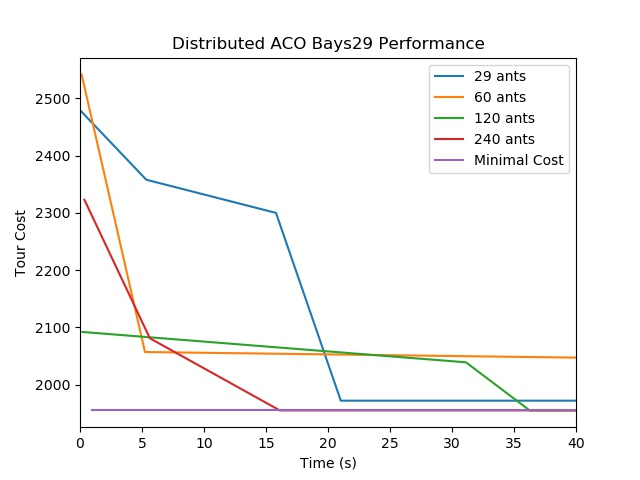
\includegraphics[scale=0.5]{bays29_performance_vs_ants.jpg}
    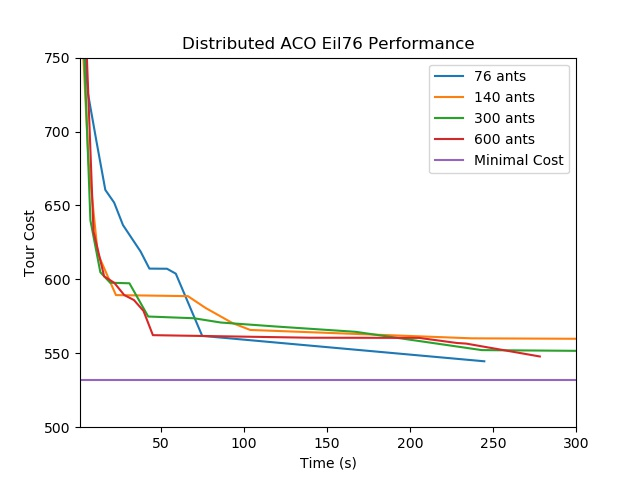
\includegraphics[scale=0.5]{eil76_performance_vs_ants.jpg}
    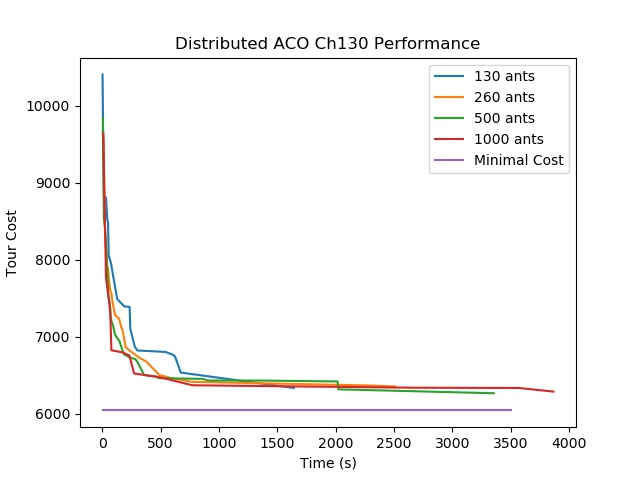
\includegraphics[scale=0.5]{ch130_performance_vs_ants.jpg}
    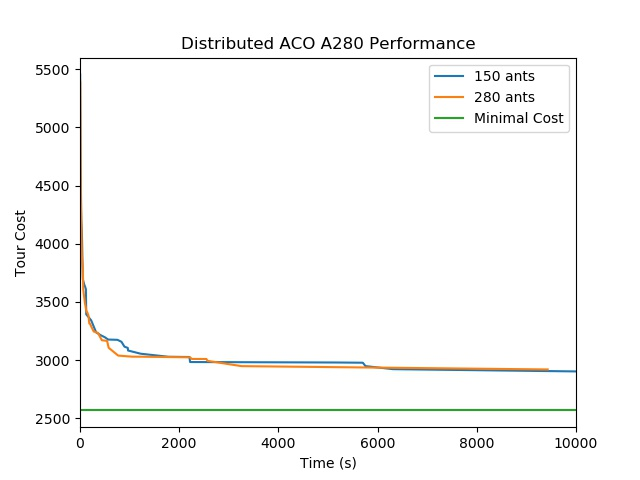
\includegraphics[scale=0.5]{a280_performance_vs_ants.jpg}
    \label{fig1}
\end{figure}


Next we turned to compare this implementation against a single threaded one. For our
experiments we ran the open sourced implementation ACOpy \cite{acopy}, which provides 
an easy to use API for running the classical ACO on problem instances from the TSPLIB95.
Figure 2 shows the progression over the four problem instances. We can see that barring 
the smallest problem size and fewest number of ants, the distributed implementation 
outperforms the serialized in all other cases in terms of cost of the optimal 
solution found, and usually in terms of time.
Note that sometimes the serialized graph goes up instead 
of down- this is a result of the API only allowing the user to specify the
amount of time for the solver to run and only providing the tour cost 
at the end of that run. Whereas data from our implementation reports from 
a single continuous run, the tour costs from the API are fragmented across
several different runs. 

\begin{figure}
    \caption{Comparing the performance of the Actor based Model against the serialized version}
    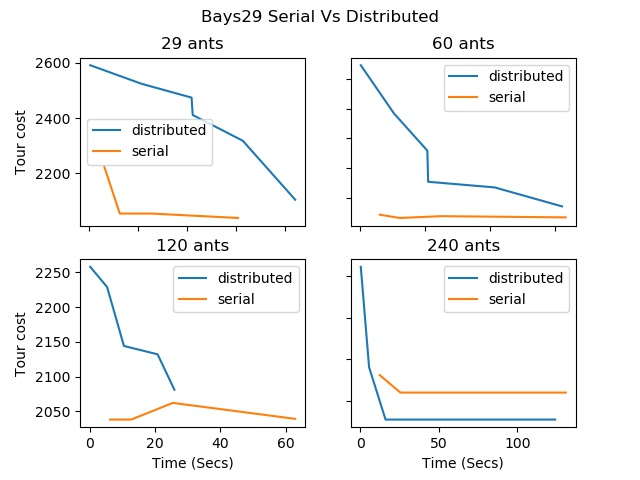
\includegraphics[scale=0.5]{bays29_serial_vs_dist.jpg}
    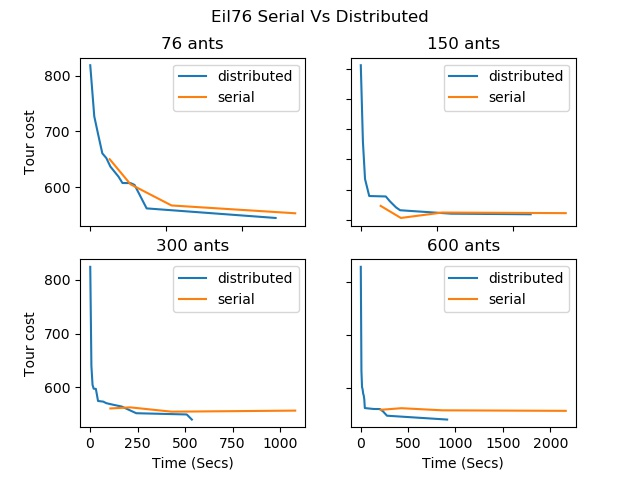
\includegraphics[scale=0.5]{eil76_serial_vs_dist.jpg}
    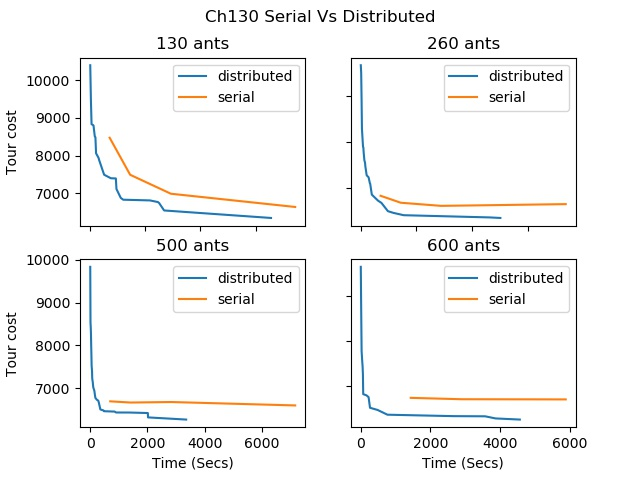
\includegraphics[scale=0.5]{ch130_serial_vs_dist.jpg}
    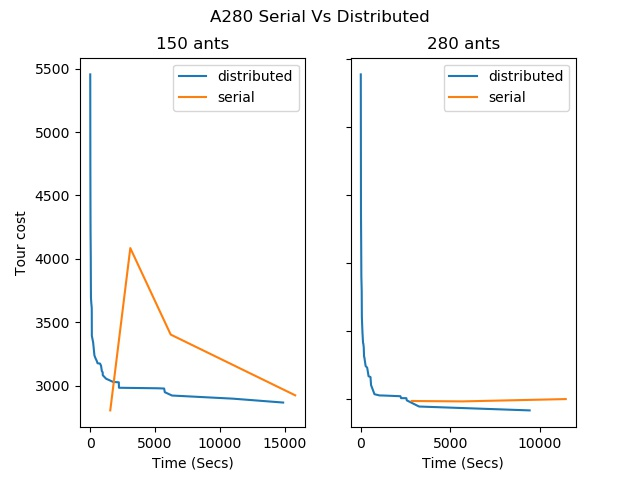
\includegraphics[scale=0.5]{a280_serial_vs_dist.jpg}
\end{figure}

\section{Future Work}
Likely apparent from the experiment set up is that the only process type with 
multiple instances spawned is the Ant process. The clear bottleneck in the 
current state of the implementation are the single Graph and Pheromone Managers. 
In fact, multiple instances of the Graph Manager could be spawned without any
change in the code besides the process id given to each ant for communicating with 
the Graph Manager. For larger graphs, it may be worth the effort and space savings 
to allocate certain portions of the graph to the different Graph Managers and route 
Edge Requests from Ants to Graph Managers accordingly. On the other hand, further work is required to increase the number 
of Pheromone Managers beyond one. Each Pheromone Manager would need to be responsible 
for only some subset of edges, and incoming Pheromone Requests would be redirected
as required. A new Pheromone Manager protocol would have to be installed for the 
different Pheromone Managers to conclude that a given round has been completed and 
transition to the next round together, before servicing new pheromone requests. Finally, 
another source of limitation in these experiments is hardware, and an increase 
in the number of compute nodes would allow for the problem size and performace benefits 
to increase.
\section{Conclusion}
In this paper we have presented a method \footnote{Code here: https://github.com/Akmalleo3/ACO} for constructing the Distributed Ant Colony Optimizer 
under the message passing paradigm. As an alternative to the shared memory model of 
concurrency, message passing provides a very natural and straightforward mechanism for 
sharing state in this problem domain. Just the simplest of clocks that 
increment with the round count capture all of the ordering that is required and reflect 
the allowed concurrency of all of the ants on their own journeys within a given round. 
Using an ActorModel language like Elixir facilitated the organization of the algorithm 
into a set of state machines (agents) and the message traffic between them. With this 
method of construction, scaling processes with size of the problem becomes practically trivial.
Best of all we found that performace under this architecture provides benefits in both speed and accuracy
over classical serialized constructions.

\clearpage
%\end{multicols*}

\bibliographystyle{plain}
\bibliography{refs}


\end{document}
